\documentclass[fleqn,10pt]{wlscirep}
\usepackage[utf8]{inputenc}
\usepackage[T1]{fontenc}
\usepackage{amsmath}
\usepackage{amssymb}
\usepackage{subcaption}
\usepackage{float}

% --- Prefix figures, tables, equations and sections with "S" ---
\renewcommand{\thefigure}{S\arabic{figure}}
\renewcommand{\thetable}{S\arabic{table}}
\renewcommand{\theequation}{S\arabic{equation}}

\title{Supplementary Information --- Advanced Machine Learning Strategies for Predicting Therapy Response in Preclinical Glioblastoma using Longitudinal MRI}

\author[1,*]{Javier González Béjar}
\author[2,3]{Ana Paula Candiota}
\author[1,3,4]{Alfredo Vellido}
\affil[1]{Universitat Politècnica de Catalunya (UPC), Department of Computer Science, Barcelona, Spain}
\affil[2]{Universitat Autònoma de Barcelona (UAB), Department of Biochemistry and Molecular Biology, Cerdanyola del Vallès, Spain}
\affil[3]{Centro de Investigación Biomédica en Red en Bioingeniería, Biomateriales y Nanomedicina (CIBER-BBN), Madrid, Spain}
\affil[4]{Intelligent Data Science and Artificial Intelligence (IDEAI) Research Center, UPC, Barcelona, Spain}

\affil[*]{javier.gonzalez.bejar@estudiantat.upc.edu}

\begin{abstract}
This document provides supplementary methods, tables, and figures supporting the main manuscript. Supplementary items are referenced in the main text as Supplementary Methods, Supplementary Tables S1--S5, and Supplementary Figures S1--S5.
\end{abstract}

\begin{document}

\flushbottom
\maketitle
\thispagestyle{empty}

\section*{Supplementary Methods}

\subsection*{EfficientNetB0 architecture and feature extraction}

EfficientNetB0 is a convolutional neural network from the EfficientNet family proposed by Tan and Le \cite{tan2020efficientnetrethinkingmodelscaling}. Conventional convolutional architectures scale one dimension of the network at a time (depth, width, or input resolution). EfficientNet instead applies \textit{compound scaling}, jointly scaling all three dimensions with a fixed set of coefficients, which yields a more favorable accuracy-to-parameter trade-off. The baseline EfficientNetB0 contains approximately 5.3 million parameters, substantially fewer than VGG16 ($\sim$138M), ResNet50 ($\sim$25M), or DenseNet121 ($\sim$8M), making it well-suited to small medical imaging datasets where over-parameterized models are prone to overfitting.

Two configurations were evaluated in this study:

\begin{itemize}
    \item \textbf{Frozen feature extractor (FE).} EfficientNetB0 was used with all layers frozen. Each preprocessed input image was passed through the network followed by a global average pooling layer. A dense layer with ReLU activation, batch normalization, and dropout produced a 256-dimensional embedding vector encoding spatial and textural patterns from the MRI scans. These embeddings were then classified with an XGBoost model under the same Grouped Leave-One-Out (GLOO) cross-validation scheme as the radiomics pipeline, enabling a direct comparison.
    \item \textbf{Fine-tuned model (FT).} The EfficientNetB0 backbone was partially unfrozen (last 50 layers trainable) and equipped with a custom binary classification head (global pooling, dense layer, batch normalization, dropout, and a final sigmoid activation). The model accepted three-channel inputs and was trained end-to-end with a reduced learning rate to adapt to domain-specific features while preserving low-level ImageNet representations.
\end{itemize}

All images were converted to the TFRecord format and processed through a TensorFlow \texttt{tf.data} pipeline enabling on-the-fly augmentation, shuffling, batching, and prefetching. A batch size of 32 was used as a compromise between gradient stability and computational efficiency. Random oversampling of the minority (cured) class was applied only within the training partition of each fold to avoid information leakage.

\subsection*{XGBoost classifier}

XGBoost \cite{Chen2016} is an ensemble method based on gradient-boosted decision trees. It builds an additive model in a forward stage-wise manner, at each step fitting a new tree to the negative gradient of a differentiable loss function and using a second-order Taylor approximation of the loss for more precise optimization. Regularization is achieved through L1 and L2 penalties on the leaf weights, shrinkage (learning rate), column subsampling, and tree pruning, all of which reduce overfitting in small, high-dimensional datasets.

The final hyperparameter configuration is reported in the main manuscript (radiomics XGBoost classifier configuration table). The complete grid explored during optimization is provided in Supplementary Table~\ref{tab:xgb_grid}. Class-imbalance handling strategies (SMOTE \cite{Chawla2002}, ENN \cite{Wilson1972}, and training on the original distribution) were compared, with controlled oversampling providing the best trade-off between sensitivity and specificity for the minority cured class.

\subsection*{Grad-CAM}

Gradient-weighted Class Activation Mapping (Grad-CAM) \cite{selvaraju2017gradcam} produces class-discriminative localization maps by using the gradients of the target class score with respect to the feature maps of the last convolutional layer. For a target class $c$ and feature maps $A^k$, the neuron importance weights are computed as
\begin{equation}
\alpha_k^{c} = \frac{1}{Z}\sum_{i}\sum_{j}\frac{\partial y^{c}}{\partial A^{k}_{ij}},
\end{equation}
and the localization map is obtained by a ReLU over the weighted combination of feature maps,
\begin{equation}
L^{c}_{\text{Grad-CAM}} = \text{ReLU}\!\left(\sum_{k}\alpha_k^{c} A^{k}\right).
\end{equation}
The resulting heatmaps were upsampled to the input resolution and overlaid on the original MRI to identify the anatomical regions driving each prediction. Maps were generated for both correctly classified and misclassified examinations.

\subsection*{Radiomic feature families and image transformations}

A total of 1,218 features were extracted per image using PyRadiomics \cite{pyradiomics}, following the Image Biomarker Standardization Initiative (IBSI) recommendations \cite{Zwanenburg_2020}. The feature families were:

\begin{itemize}
\item \textbf{First-order statistics}: mean, variance, entropy, skewness, kurtosis, energy, and related intensity descriptors.
\item \textbf{Shape-based descriptors}: elongation, compactness, sphericity, and surface-area-related measurements, independent of intensity.
\item \textbf{Gray-Level Co-occurrence Matrix (GLCM)}: second-order texture features quantifying spatial relationships between neighboring voxel intensities.
\item \textbf{Gray-Level Run-Length Matrix (GLRLM)}: distribution of consecutive runs of similar gray levels.
\item \textbf{Gray-Level Size-Zone Matrix (GLSZM)}: homogeneous intensity zones capturing regional heterogeneity.
\item \textbf{Gray-Level Dependence Matrix (GLDM)}: local gray-level dependencies and neighborhood homogeneity.
\item \textbf{Neighboring Gray-Tone Difference Matrix (NGTDM)}: coarseness, complexity, and contrast.
\end{itemize}

Features were computed on the original images and on multiple transformed representations: Laplacian-of-Gaussian (LoG) filtered images ($\sigma = 1.0, 2.0, 3.0$), one-level wavelet decompositions (eight frequency-specific sub-bands), gradient images, and intensity transformations (square, square-root, logarithmic, and exponential). Temporal descriptors (first-order differences, rolling means and standard deviations, local slopes, and relative percentage changes) were subsequently derived from the retained features to encode longitudinal dynamics without modeling complete sequences as a jointly classified multivariate time series.

\section*{Supplementary Tables}

\begin{table}[H]
\centering
\renewcommand{\arraystretch}{1.3}
\resizebox{\textwidth}{!}{%
\begin{tabular}{|c|c|c|c|c|}
\hline
\textbf{Code} & \textbf{Group} & \textbf{Images per Exploration} & \textbf{Number of Explorations} & \textbf{Range of Days Studied} \\
\hline
C1258 & Control & 1--3 & 6 & 7--24 \\
C1260 & Control & 1--4 & 6 & 8--18 \\
C1261 & Control & 1--5 & 8 & 10--26 \\
C1297 & Control & 2 & 1 & 23 \\
C1299 & Control & 2 & 1 & 17 \\
C1359 & Control & 1--4 & 3 & 11--16 \\
C1360 & Control & 1--4 & 6 & 11--22 \\
C1361 & Control & 1--4 & 5 & 11--20 \\
\hline
C1276 & TMZ-Treated -- Cured & 1--2 & 15 & 11--45 \\
C1281 & TMZ-Treated -- Cured & 1--2 & 8 & 10--27 \\
C1284 & TMZ-Treated -- Cured & 1 & 8 & 10--27 \\
C1285 & TMZ-Treated -- Cured & 1--2 & 10 & 9--31 \\
C1382 & TMZ-Treated -- Cured & 1 & 8 & 11--29 \\
\hline
C1263 & TMZ-Treated -- Relapsing & 1--4 & 18 & 11--47 \\
C1264 & TMZ-Treated -- Relapsing & 1--4 & 16 & 11--39 \\
C1270 & TMZ-Treated -- Relapsing & 1--4 & 14 & 10--37 \\
C1380 & TMZ-Treated -- Relapsing & 1--4 & 17 & 11--41 \\
C1383 & TMZ-Treated -- Relapsing & 1--4 & 19 & 11--49 \\
\hline
\end{tabular}%
}
\caption{Per-subject description of the dataset. Each row corresponds to one animal, identified by a unique code (CXXXX). Columns report the group, the number of MRI images acquired at each time point, the number of explorations (imaging sessions) performed over time, and the range of days studied, taking day 0 as the tumor inoculation day.}
\label{tab:subjects}
\end{table}

\begin{table}[H]
\centering
\begin{tabular}{ll}
\hline
Hyperparameter & Values explored \\
\hline
\texttt{max\_depth} & \{2, 3, 4, 5\} \\
\texttt{learning\_rate} & \{0.01, 0.05, 0.1\} \\
\texttt{n\_estimators} & \{100, 200, 300\} \\
\texttt{min\_child\_weight} & \{1, 3, 5\} \\
\texttt{gamma} & \{0, 0.5, 1\} \\
\texttt{subsample} & \{0.6, 0.8, 1.0\} \\
\texttt{colsample\_bytree} & \{0.6, 0.8, 1.0\} \\
Resampling & \{none, SMOTE, ENN\} \\
\hline
\end{tabular}
\caption{Hyperparameter search grid for the radiomics-based XGBoost classifier. The final configuration selected by cross-validation is reported in Supplementary Table~S3.}
\label{tab:xgb_grid}
\end{table}

\begin{table}[H]
\centering
\begin{tabular}{ll}
\hline
Parameter & Value \\
\hline
Base learner & Gradient-boosted decision trees \\
\texttt{max\_depth} & 3 \\
\texttt{learning\_rate} & 0.01 \\
\texttt{n\_estimators} & 100 \\
\texttt{subsample} & 0.6 \\
\texttt{colsample\_bytree} & 0.6 \\
\texttt{gamma} & 0.5 \\
Regularization & L1 and L2 penalties \\
Class-imbalance handling & SMOTE / ENN / none (compared) \\
Hyperparameter search & Grid search (see Supplementary Table~S2) \\
Validation & Grouped Leave-One-Out (GLOO) \\
\hline
\end{tabular}
\caption{Final configuration of the radiomics-based XGBoost classifier.}
\label{tab:ml_params}
\end{table}

\begin{table}[H]
\centering
\begin{tabular}{ll}
\hline
Parameter & Value \\
\hline
Backbone & EfficientNetB0 (ImageNet pre-trained) \\
Trainable layers & Last 50 layers unfrozen \\
Input & 3-channel images \\
Classification head & Global pooling + dense + batch norm + dropout + sigmoid \\
Loss function & Binary cross-entropy \\
Optimizer & Adam \\
Batch size & 32 \\
Class-imbalance handling & Random oversampling (training folds only) \\
Regularization & Dropout, early stopping \\
Validation & Grouped Leave-One-Out (GLOO) \\
\hline
\end{tabular}
\caption{Configuration of the EfficientNetB0 fine-tuning procedure.}
\label{tab:dl_params}
\end{table}

\section*{Supplementary Figures}

\begin{figure}[H]
\centering
\begin{subfigure}[b]{0.6\textwidth}
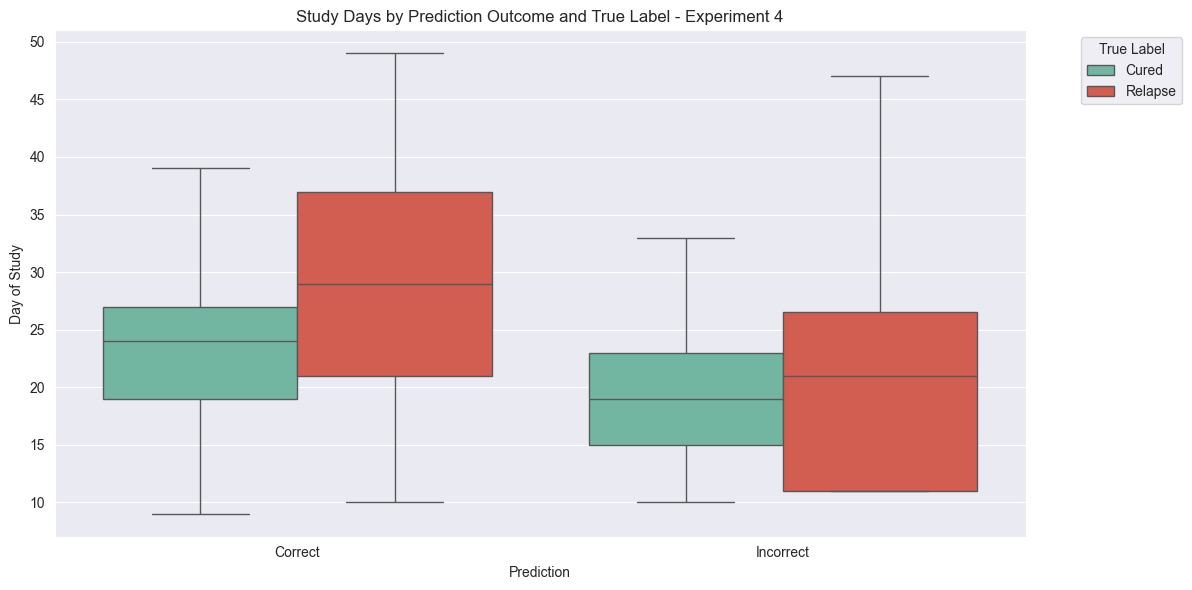
\includegraphics[width=\textwidth]{images/boxplot-exp4.png}
\caption{Configuration 4}
\end{subfigure}
\hfill
\begin{subfigure}[b]{0.6\textwidth}
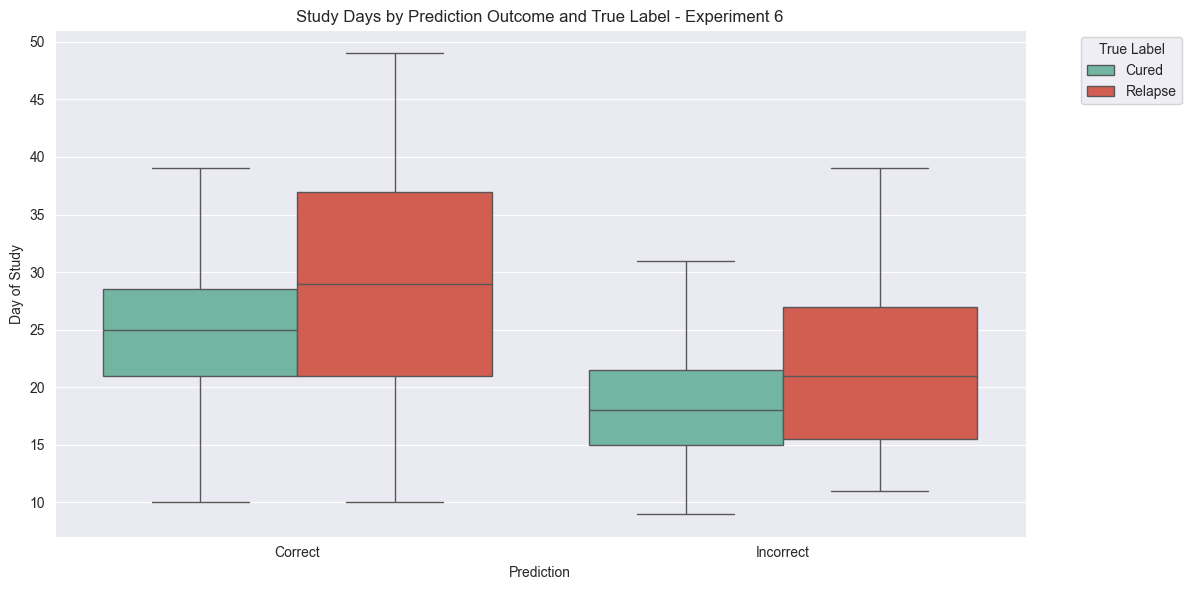
\includegraphics[width=\textwidth]{images/boxplot-exp6.png}
\caption{Configuration 6}
\end{subfigure}
\hfill
\begin{subfigure}[b]{0.6\textwidth}
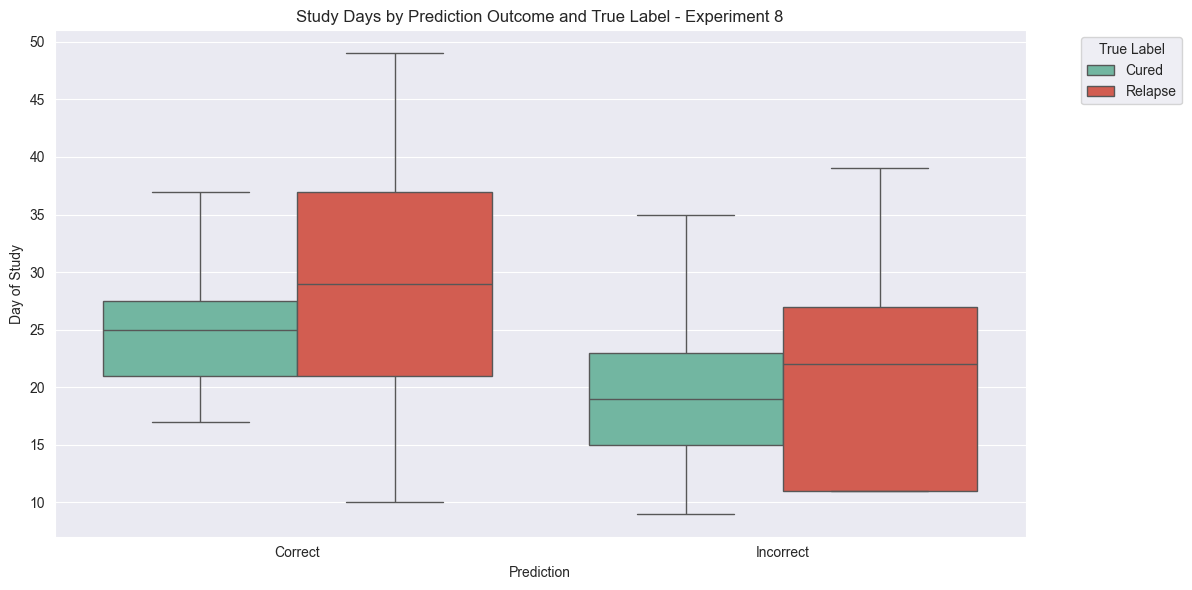
\includegraphics[width=\textwidth]{images/boxplot-exp8.png}
\caption{Configuration 8}
\end{subfigure}
\caption{Distribution of cross-validation performance for representative radiomics configurations, illustrating the effect of the different class-imbalance handling strategies (original distribution, SMOTE, and ENN) on the XGBoost classifier.}
\label{fig:sfig_boxplots}
\end{figure}

\begin{figure}[H]
\centering
\begin{subfigure}[b]{0.75\textwidth}
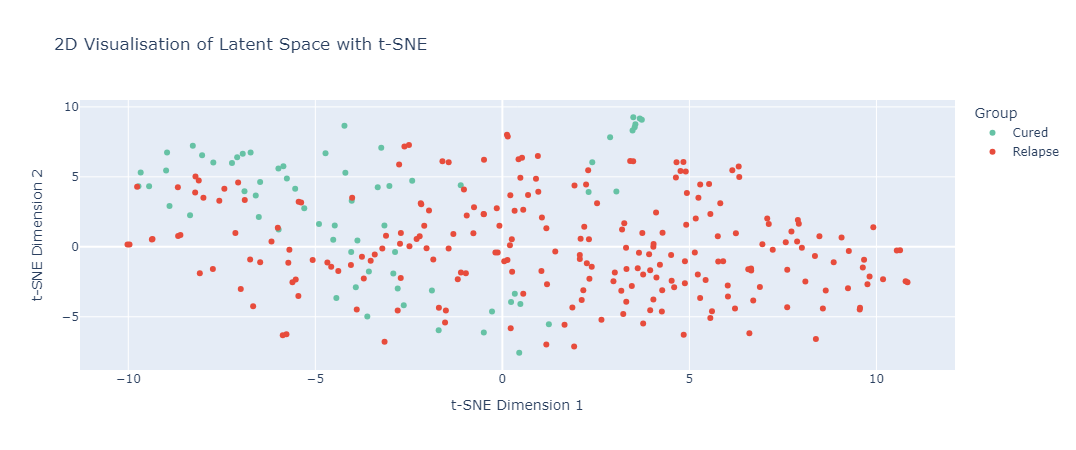
\includegraphics[width=\textwidth]{images/tsne.png}
\caption{t-SNE projection}
\end{subfigure}
\hfill
\begin{subfigure}[b]{0.75\textwidth}
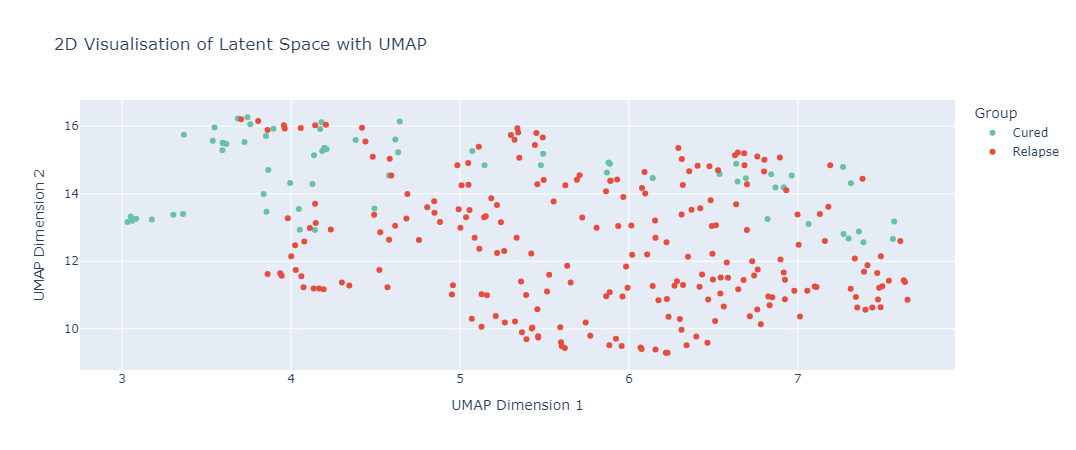
\includegraphics[width=\textwidth]{images/umap.png}
\caption{UMAP projection}
\end{subfigure}
\caption{Low-dimensional projections (t-SNE and UMAP) of the selected radiomic feature space, colored by outcome group. These visualizations illustrate the partial separability between cured and relapsing examinations.}
\label{fig:sfig_latent}
\end{figure}

\begin{figure}[H]
\centering
\begin{subfigure}[b]{0.75\textwidth}
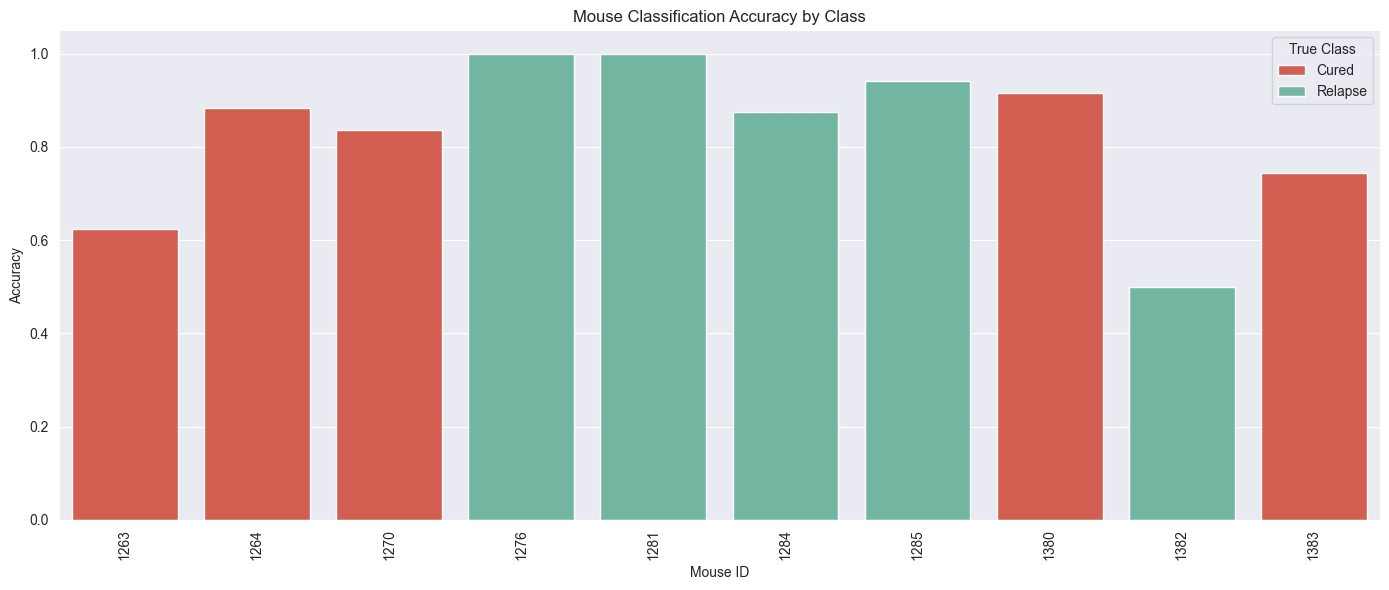
\includegraphics[width=\textwidth]{images/m_classification_accuracy_by_class.png}
\caption{Classification accuracy by class}
\end{subfigure}
\hfill
\begin{subfigure}[b]{0.75\textwidth}
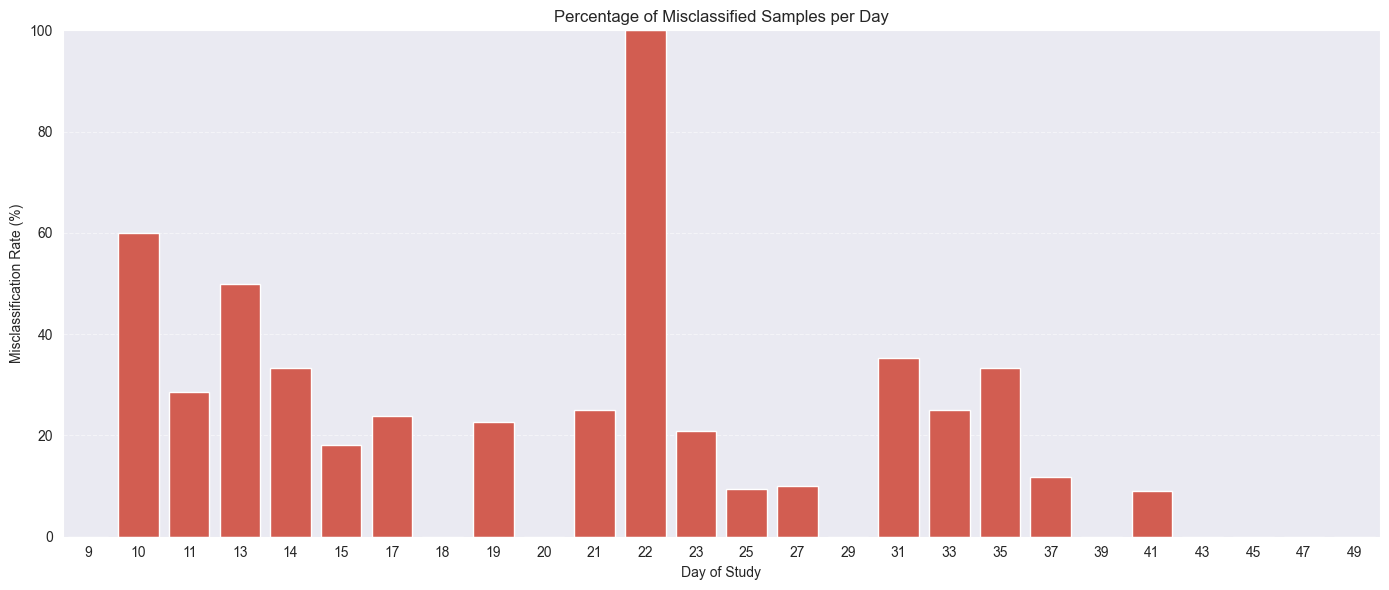
\includegraphics[width=\textwidth]{images/misclassified_samples_per_day.png}
\caption{Misclassified examinations per day}
\end{subfigure}
\caption{Temporal analysis of predictive performance for the deep learning model. (a) Classification accuracy per class and (b) number of misclassified examinations as a function of tumor evolution day, showing reduced performance at the earliest time points.}
\label{fig:sfig_temporal}
\end{figure}

\begin{figure}[H]
\centering
\begin{subfigure}[b]{0.32\textwidth}
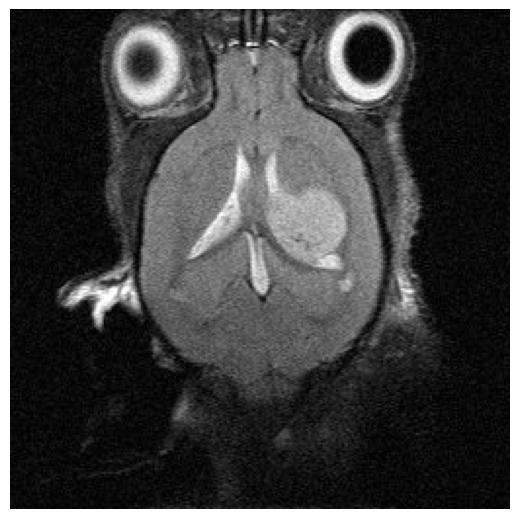
\includegraphics[width=\textwidth]{images/1263_d14_mri.png}
\caption{Day 14 -- MRI}
\end{subfigure}
\hfill
\begin{subfigure}[b]{0.32\textwidth}
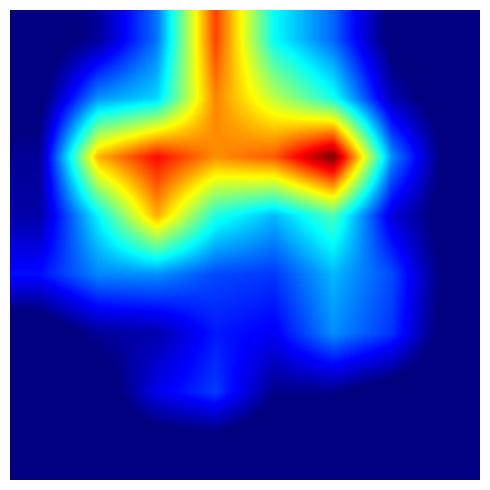
\includegraphics[width=\textwidth]{images/1263_d14_heat.png}
\caption{Day 14 -- Heatmap}
\end{subfigure}
\hfill
\begin{subfigure}[b]{0.32\textwidth}
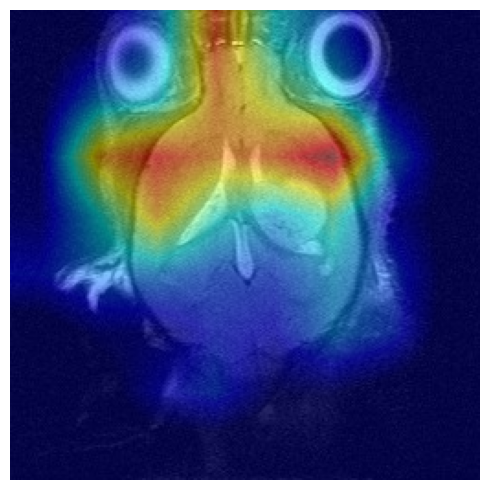
\includegraphics[width=\textwidth]{images/1263_d14_gradcam.png}
\caption{Day 14 -- Grad-CAM}
\end{subfigure}

\vspace{2mm}

\begin{subfigure}[b]{0.32\textwidth}
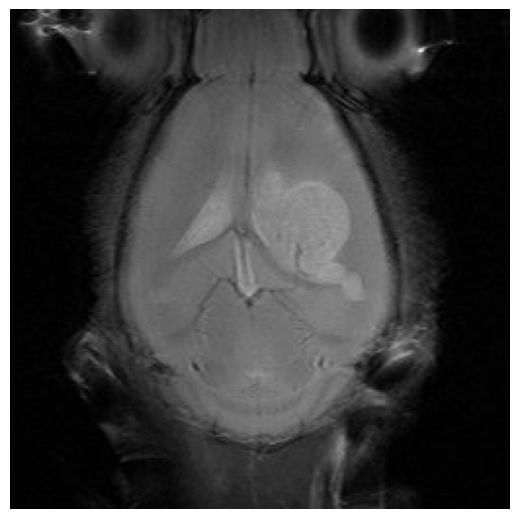
\includegraphics[width=\textwidth]{images/1263_d17_mri.png}
\caption{Day 17 -- MRI}
\end{subfigure}
\hfill
\begin{subfigure}[b]{0.32\textwidth}
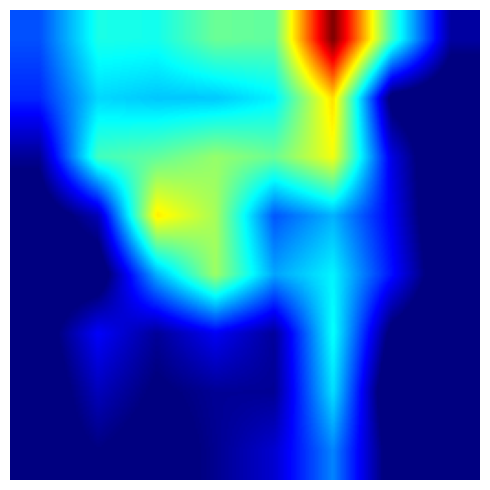
\includegraphics[width=\textwidth]{images/1263_d17_heat.png}
\caption{Day 17 -- Heatmap}
\end{subfigure}
\hfill
\begin{subfigure}[b]{0.32\textwidth}
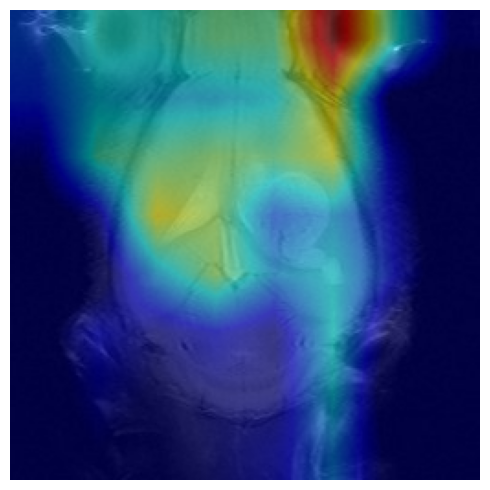
\includegraphics[width=\textwidth]{images/1263_d17_gradcam.png}
\caption{Day 17 -- Grad-CAM}
\end{subfigure}

\vspace{2mm}

\begin{subfigure}[b]{0.32\textwidth}
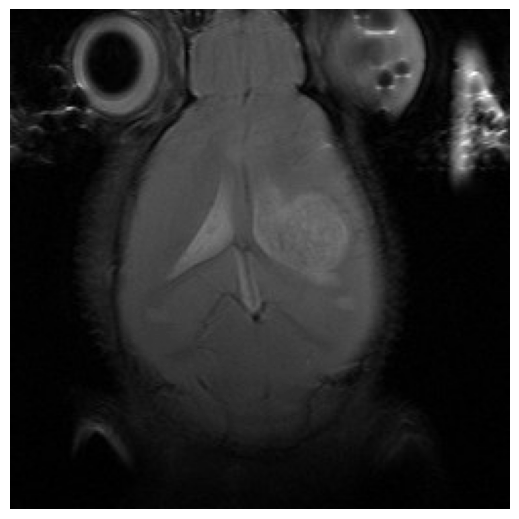
\includegraphics[width=\textwidth]{images/1263_d19_mri.png}
\caption{Day 19 -- MRI}
\end{subfigure}
\hfill
\begin{subfigure}[b]{0.32\textwidth}
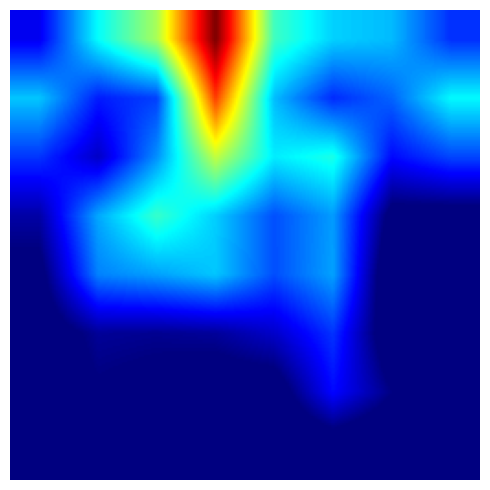
\includegraphics[width=\textwidth]{images/1263_d19_heat.png}
\caption{Day 19 -- Heatmap}
\end{subfigure}
\hfill
\begin{subfigure}[b]{0.32\textwidth}
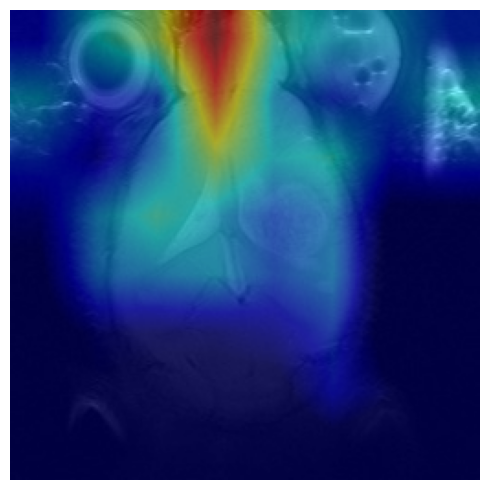
\includegraphics[width=\textwidth]{images/1263_d19_gradcam.png}
\caption{Day 19 -- Grad-CAM}
\end{subfigure}
\caption{Temporal evolution of Grad-CAM attention maps for subject C1263 across days 14, 17, and 19, complementing the day-11 visualization shown in the main manuscript. Each row shows the original MRI, the Grad-CAM heatmap, and the overlay.}
\label{fig:sfig_gradcam_evolution}
\end{figure}

\begin{figure}[H]
\centering
\begin{subfigure}[b]{0.45\textwidth}
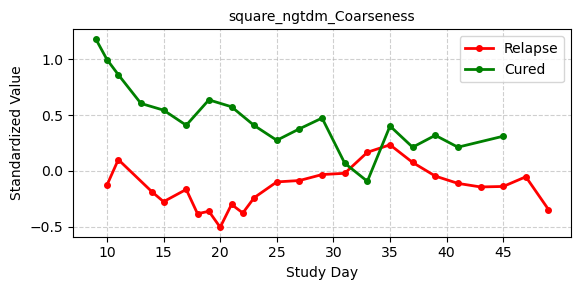
\includegraphics[width=\textwidth]{images/coarseness.png}
\caption{Coarseness}
\end{subfigure}
\hfill
\begin{subfigure}[b]{0.45\textwidth}
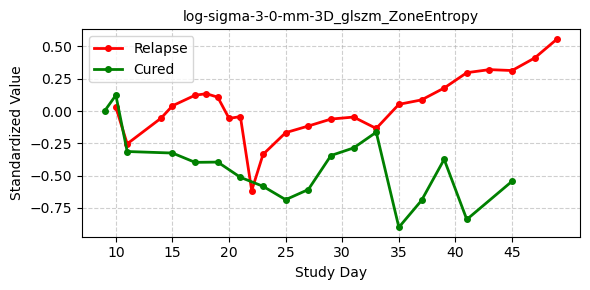
\includegraphics[width=\textwidth]{images/zoneentropy.png}
\caption{Zone Entropy}
\end{subfigure}
%\hfill
\vspace{2mm}
\begin{subfigure}[b]{0.45\textwidth}
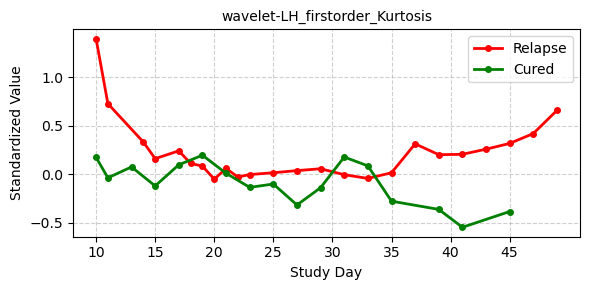
\includegraphics[width=\textwidth]{images/kurtosis.png}
\caption{Kurtosis}
\end{subfigure}
\hfill
%\vspace{2mm}
\begin{subfigure}[b]{0.45\textwidth}
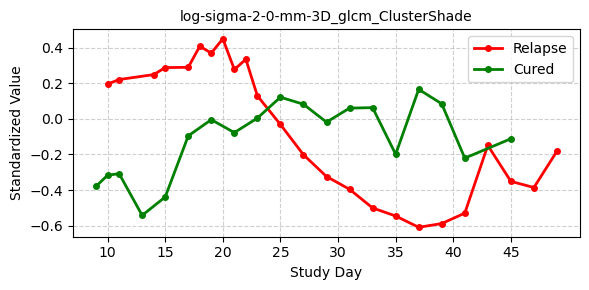
\includegraphics[width=\textwidth]{images/clustershade.png}
\caption{Cluster Shade}
\end{subfigure}
%\hfill
\vspace{2mm}

\begin{subfigure}[b]{0.45\textwidth}
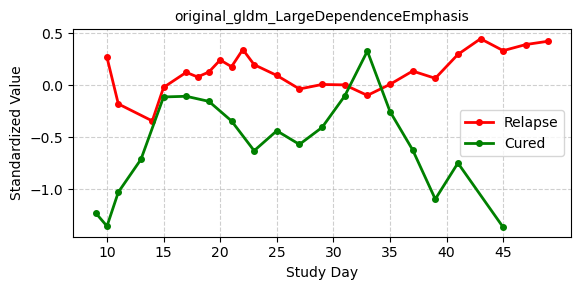
\includegraphics[width=\textwidth]{images/largedependenceemphasis.png}
\caption{Large Dependence Emphasis}
\end{subfigure}
\hfill
\begin{subfigure}[b]{0.45\textwidth}
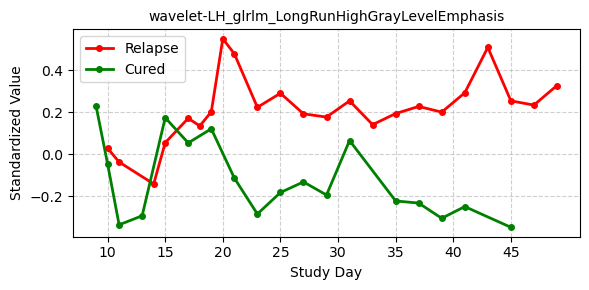
\includegraphics[width=\textwidth]{images/longrunhighlevelemphasis.png}
\caption{Long Run High Gray Level Emphasis}
\end{subfigure}
\caption{Temporal evolution of additional selected radiomic features across cured and relapsing groups, complementing the Elongation and Dependence Entropy trajectories shown in the main text.}
\label{fig:sfig_extra_features}
\end{figure}

\section*{Supplementary Table S5 --- Animal-Level Majority-Vote Results}

Table~\ref{tab:animal_level} reports subject-level predictions obtained by majority vote across all MRI examinations for each treated animal. For each animal, the predicted class is the most frequent exam-level prediction; the mean predicted probability is averaged across all examinations of that animal. All three pipelines correctly identified all five relapsing animals (Specificity~=~1.00). The two cured animals consistently misclassified across all pipelines (C1285 and C1382) suggest that their imaging signatures overlap more with the relapsing group throughout the follow-up.

\begin{table}[H]
\centering
\caption{Animal-level classification results (majority vote across examinations) for all three pipelines. True outcome: 0 = relapsing, 1 = cured. Predicted: 0 = relapsing, 1 = cured. Mean prob. = mean predicted probability of cure averaged across all examinations of that animal. Correct predictions are marked with \checkmark; errors with $\times$.}
\label{tab:animal_level}
\begin{tabular}{lcccccccc}
\hline
 & & & \multicolumn{2}{c}{Radiomics} & \multicolumn{2}{c}{Eff.\ FE+XGB} & \multicolumn{2}{c}{Eff.\ FT} \\
\cmidrule(lr){4-5}\cmidrule(lr){6-7}\cmidrule(lr){8-9}
Animal & Outcome & N exams & Pred & Mean prob. & Pred & Mean prob. & Pred & Mean prob. \\
\hline
C1263 & Relapsing & 56 & 0\ \checkmark & 0.419 & 0\ \checkmark & 0.390 & 0\ \checkmark & 0.401 \\
C1264 & Relapsing & 43 & 0\ \checkmark & 0.367 & 0\ \checkmark & 0.316 & 0\ \checkmark & 0.413 \\
C1270 & Relapsing & 43 & 0\ \checkmark & 0.295 & 0\ \checkmark & 0.315 & 0\ \checkmark & 0.282 \\
C1380 & Relapsing & 47 & 0\ \checkmark & 0.306 & 0\ \checkmark & 0.295 & 0\ \checkmark & 0.147 \\
C1383 & Relapsing & 43 & 0\ \checkmark & 0.400 & 0\ \checkmark & 0.404 & 0\ \checkmark & 0.483 \\
\hline
C1276 & Cured & 21 & 1\ \checkmark & 0.534 & 1\ \checkmark & 0.604 & 1\ \checkmark & 0.904 \\
C1281 & Cured & 12 & 1\ \checkmark & 0.638 & 1\ \checkmark & 0.594 & 1\ \checkmark & 0.979 \\
C1284 & Cured &  8 & 1\ \checkmark & 0.657 & 1\ \checkmark & 0.624 & 1\ \checkmark & 0.949 \\
C1285 & Cured & 17 & 0\ $\times$ & 0.417 & 0\ $\times$ & 0.476 & 1\ \checkmark & 0.632 \\
C1382 & Cured &  8 & 0\ $\times$ & 0.415 & 0\ $\times$ & 0.347 & 0\ $\times$ & 0.399 \\
\hline
\multicolumn{3}{l}{AUC (animal-level)} & \multicolumn{2}{c}{0.92} & \multicolumn{2}{c}{0.92} & \multicolumn{2}{c}{0.88} \\
\multicolumn{3}{l}{Sensitivity} & \multicolumn{2}{c}{0.60} & \multicolumn{2}{c}{0.60} & \multicolumn{2}{c}{0.80} \\
\multicolumn{3}{l}{Specificity} & \multicolumn{2}{c}{1.00} & \multicolumn{2}{c}{1.00} & \multicolumn{2}{c}{1.00} \\
\multicolumn{3}{l}{Accuracy} & \multicolumn{2}{c}{0.80} & \multicolumn{2}{c}{0.80} & \multicolumn{2}{c}{0.90} \\
\hline
\end{tabular}
\end{table}

\bibliography{refs}

\end{document}
